\documentclass[twocolumn]{article}
\usepackage{listings}
\usepackage{booktabs}
\usepackage{here}
\usepackage{subcaption}
\usepackage{tikz}
\usepackage{amsmath}
\usepackage{graphicx}
\usepackage{hyperref}
\usepackage{siunitx} % Required for the \num command
\usepackage{float}

\newcommand{\code}[1]{{\tt #1}}

% decreas margin size
\usepackage[margin=0.7in]{geometry}

\newcommand\blankpage{%
	\null
	\thispagestyle{empty}%
	\addtocounter{page}{-1}%
	\newpage}

\title{
	\normalfont\normalsize
	\textsc{Robotics SP 2025\\
	Universit\`a della Svizzera italiana}\\
	% \vspace{2pt}
	\rule{\linewidth}{0.5pt}\\
	% \vspace{5pt}
	{\huge Tower Dropper\\
	\small Group Z}\\
	% \vspace{5pt}
	\rule{\linewidth}{1pt}\\
	\vspace{5pt}
}

\author{
	Paolo Deidda (\text{paolo.deidda@usi.ch}) \\ 
	Francesco Costa (\text{francesco.costa@usi.ch})\\
	Raffaele Perri (\text{raffaele.perri@usi.ch})\\
	\url{https://github.com/USI-Projects-Collection/FinalProject-Robotics.git}
	}
\begin{document}
\begin{titlepage}
    \begin{center}
        \textsc{Robotics SP 2025\\
        Universit\`a della Svizzera italiana}\\[1ex]
        
        \rule{\linewidth}{0.5pt}\\[1ex]
        {\huge Tower Dropper\\[0.5ex]
        \small Group Z}\\[1ex]
        \rule{\linewidth}{1pt}\\[2ex]

        \normalsize
        Paolo Deidda (\texttt{paolo.deidda@usi.ch})\\
        Francesco Costa (\texttt{francesco.costa@usi.ch})\\
        Raffaele Perri (\texttt{raffaele.perri@usi.ch})\\[1ex]
        \url{https://github.com/USI-Projects-Collection/FinalProject-Robotics.git}
    \end{center}

    \vspace{2em}
    \tableofcontents

    \vspace{2em}
    \subsection*{Setup}
    To run the code follow the setup and execution instructions provided in the \texttt{README.md} file included in this repository.
\end{titlepage}

% ====================================================================
\section{Introduction}\label{sec:intro}
\subsection{Model and Scene}
The project use a RobomasterS1 robot model, with the addition of four proximity sensors, placed respectively (Figure~\ref{fig:robot_model}):
\begin{itemize}
\item \textbf{Range\_0 (Center-right)}: Primary sensor for orbit distance maintenance during left-side orbital maneuvers. Positioned at the robot's right quadrant with a detection range up to 10 meters.
\item \textbf{Range\_1 (Front-right)}: Primary sensor for initial tower detection and forward-right obstacle detection. Critical for the search phase and collision avoidance.
\item \textbf{Range\_2 (Center-left)}: Secondary sensor utilized during obstacle avoidance protocols, enabling the robot to maintain safe distances from obstacles while navigating around them.
\item \textbf{Range\_3 (Front-left)}: Forward collision prevention sensor that triggers emergency avoidance behaviors when obstacles are detected within critical thresholds.
\end{itemize}
\begin{figure}[H]
    \centering
    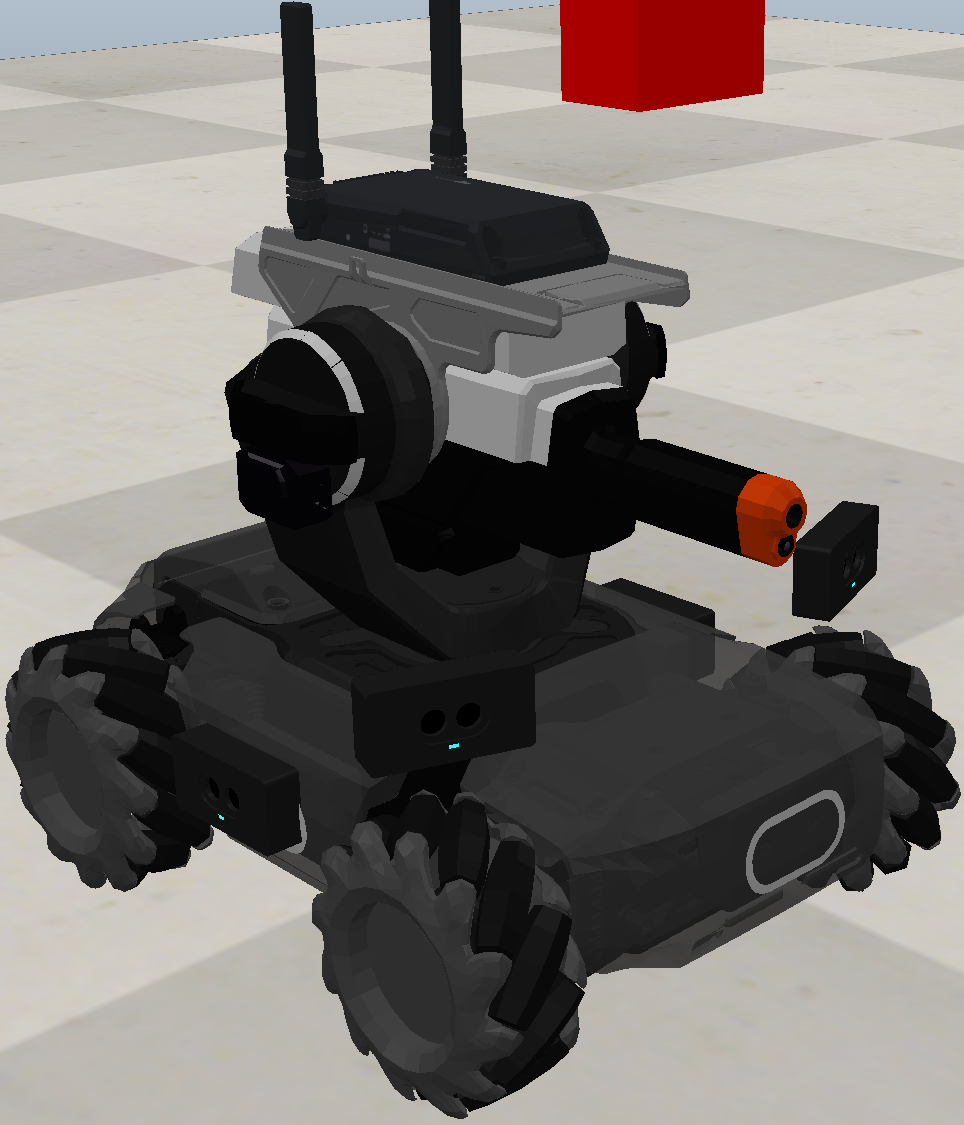
\includegraphics[width=0.2\textwidth]{Images/RobomasterS1_model.png}
    \caption{RobomasterS1 robot model with camera and proximity sensors.}
    \label{fig:robot_model}
\end{figure}
The robot is equipped with a camera (\texttt{/rm0/camera/image\_color}) used for visual processing tasks, such as weak-spot detection and tower identification.\\
The scene is constructed with a 3D model of the RobomasterS1 robot placed in the center of a flat terrain. The environment includes four towers, each colored in red to indicate that they are active and can be targeted. The towers are positioned at the corners of the scene (\text{ADD SOME OTHER DETAILS ABOUT THE SCENE}).\\
\textbf{ADD A PICTURE OF THE SCENE HERE.}\\

% ====================================================================
\section{Workflow of the Project}\label{sec:workflow}
\subsection{Global Path Planning}\label{sec:planner}
\subsubsection{Objectives and Requirements}
The goal of our global planner is to compute, at runtime, a collision-free route from the robot’s current pose to the next tower in the Tower Dropper scenario. The planner must respect:
\begin{itemize}
  \item \textbf{Static environment:} a 5\,m × 5\,m occupancy grid (5\,cm resolution) generated by our mock map publisher.
  \item \textbf{Robot footprint:} approximated as a circle of radius 0.3\,m, enforced via obstacle inflation.
  \item \textbf{Real-time constraints:} paths should be available within a few hundred milliseconds to allow seamless integration with our local controller and to react promptly when the mock publisher advances to the next tower.
\end{itemize}

\subsubsection{Algorithm Selection and Design}
We surveyed classic grid-based planners (Dijkstra for guaranteed optimality, RRT for sampling-based routes) but settled on \textbf{A*} on an occupancy grid for its simplicity and determinism. In our \texttt{PathPlannerNode}:
\begin{enumerate}
  \item \textbf{Grid representation:} a 2D \texttt{NumPy} array of occupancy values (0 = free, $\geq$50 = occupied).
  \item \textbf{Search:} an 8-connected A* using a min-heap (\texttt{heapq}) keyed by $f = g + h$, where $g$ is accumulated path cost and $h$ the Euclidean distance to goal. Orthogonal moves cost 1; diagonal moves cost $\sqrt{2}$. Corner-cutting checks prevent invalid diagonals.
  \item \textbf{Path pruning:} after finding the raw A* path, we remove unnecessary waypoints by testing straight-line visibility with a Bresenham-based \texttt{\_has\_los} check.
\end{enumerate}

\subsubsection{Map Representation, Visualization \& Preprocessing}
To debug and tune our planner, we relied heavily on \texttt{RViz2}, subscribing to the \texttt{/map} and \texttt{/plan} topics to inspect both the occupancy grid and computed paths in real time. Figures~\ref{fig:raw-pruned} and~\ref{fig:inflated} illustrate this process.

\begin{figure}[ht]
  \centering
  \begin{minipage}[b]{0.24\textwidth}
    \centering
    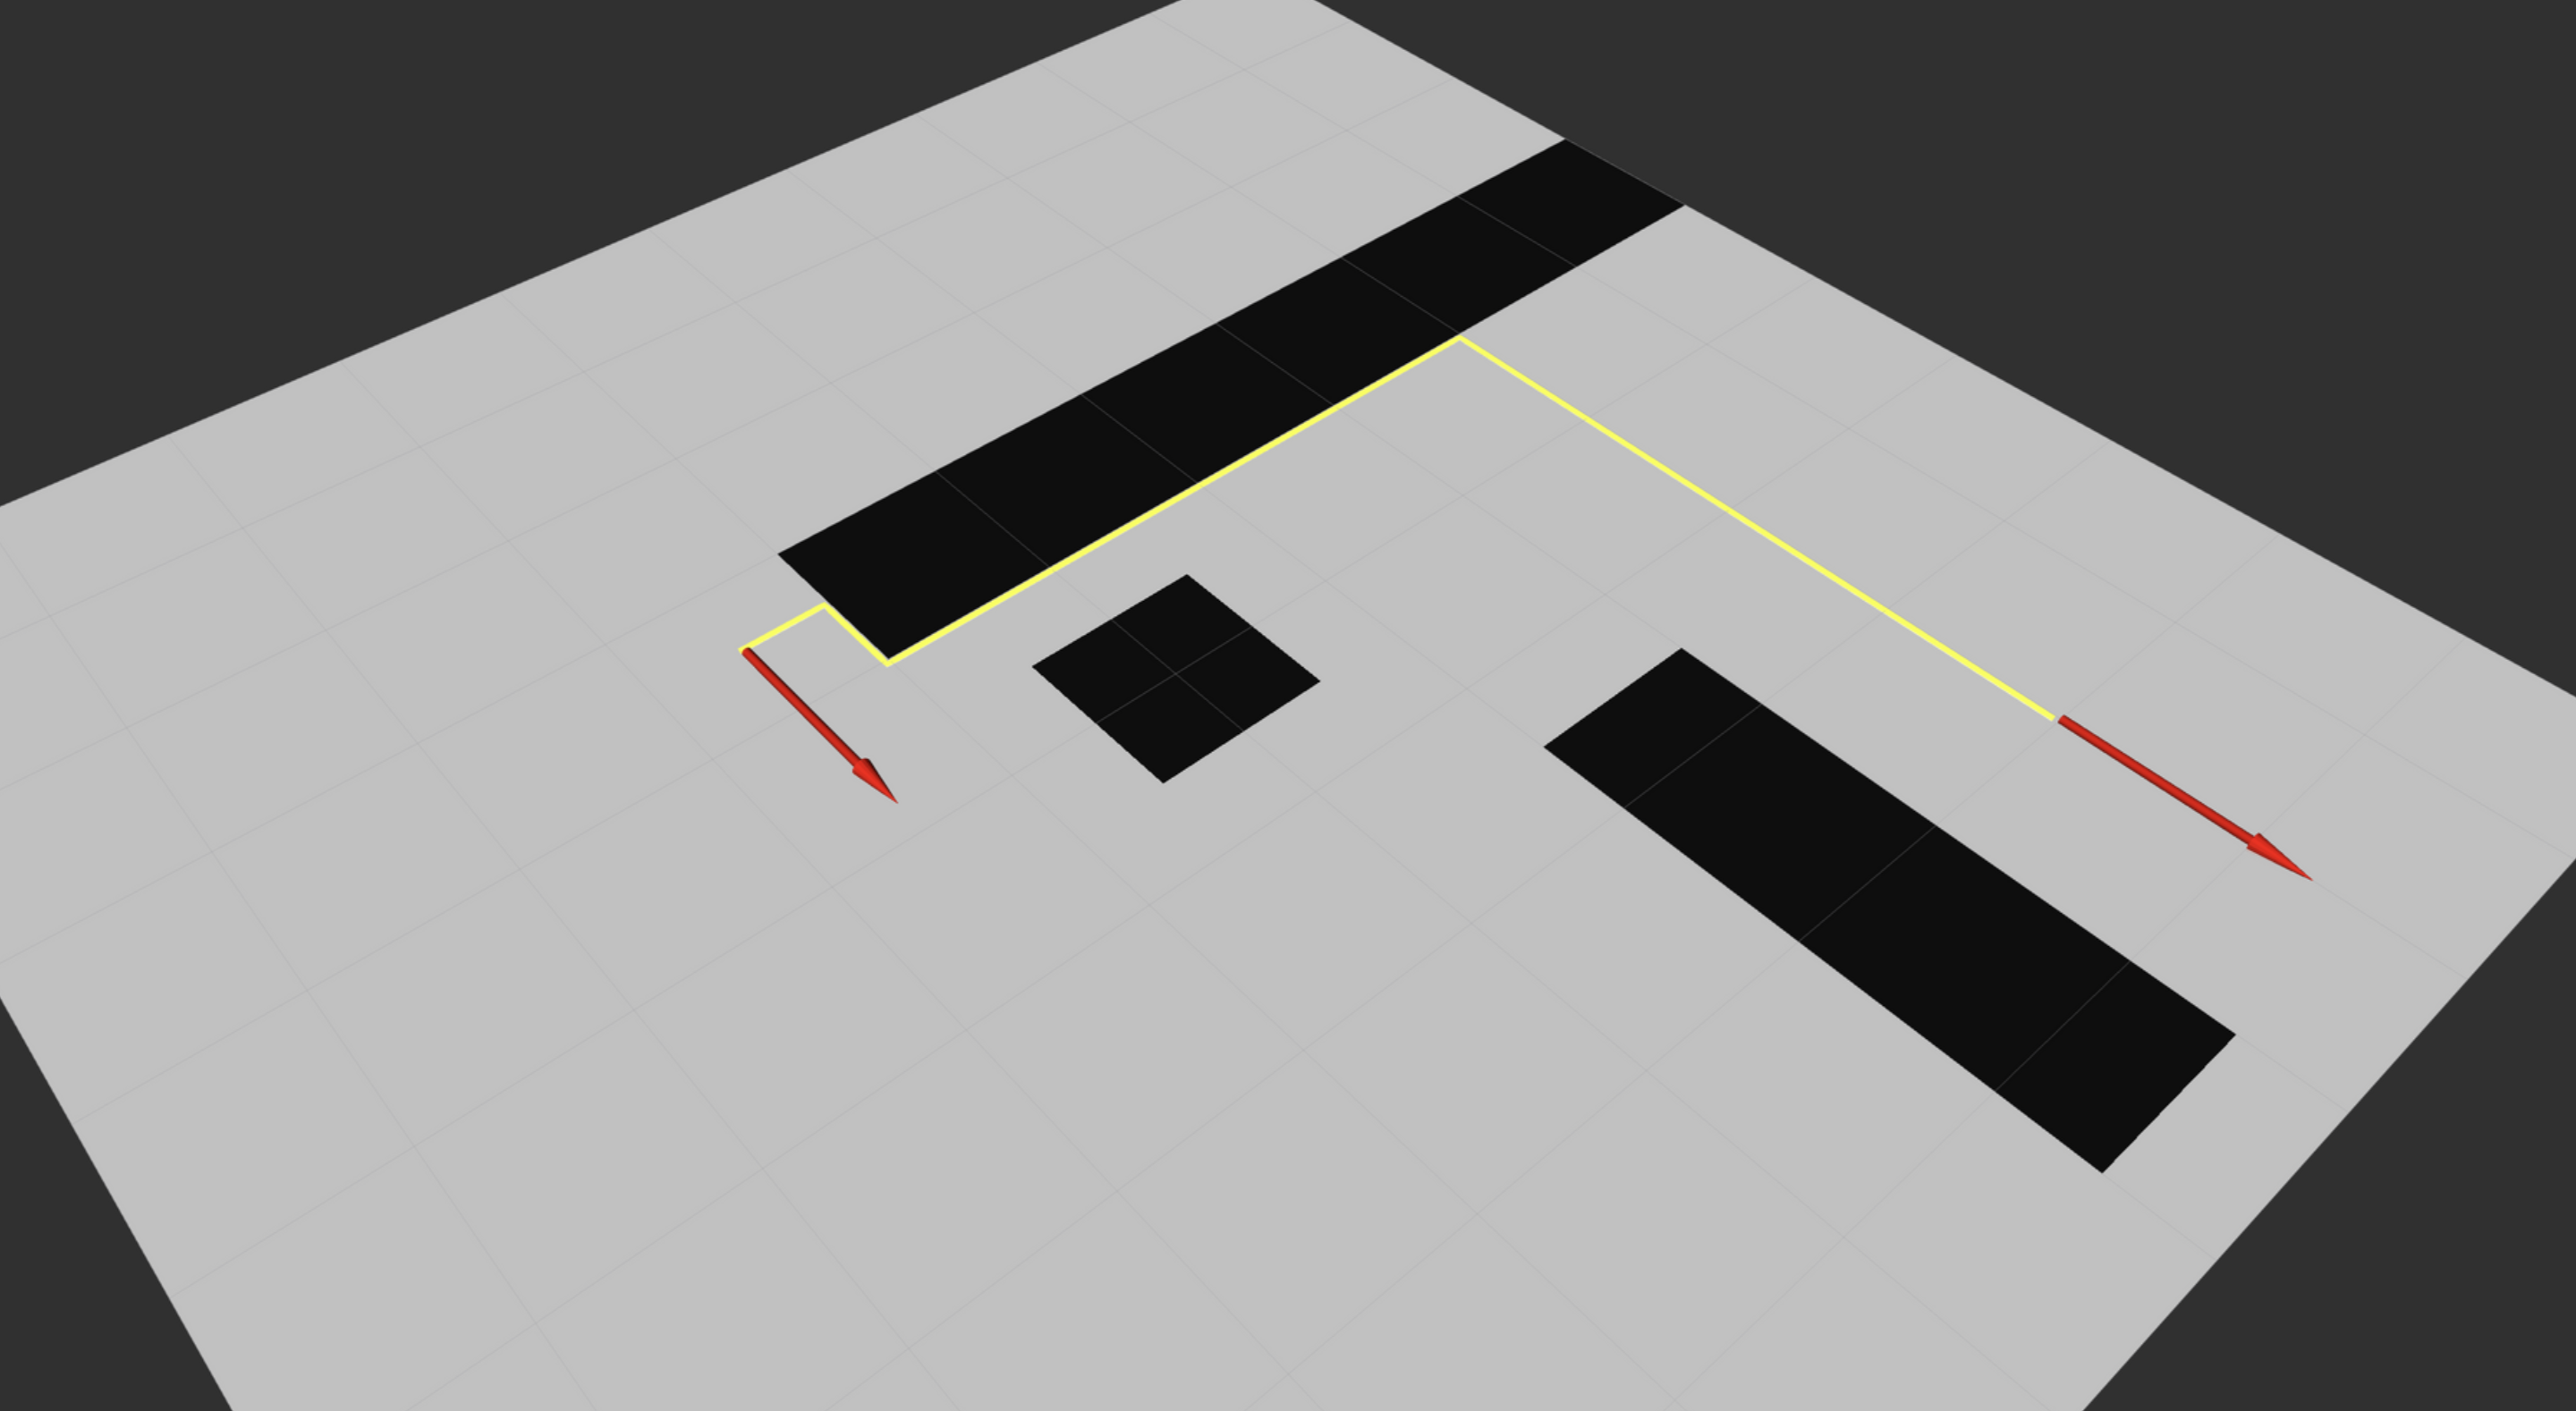
\includegraphics[width=\linewidth]{Images/path1.png}
  \end{minipage}
  \hfill
  \begin{minipage}[b]{0.24\textwidth}
    \centering
    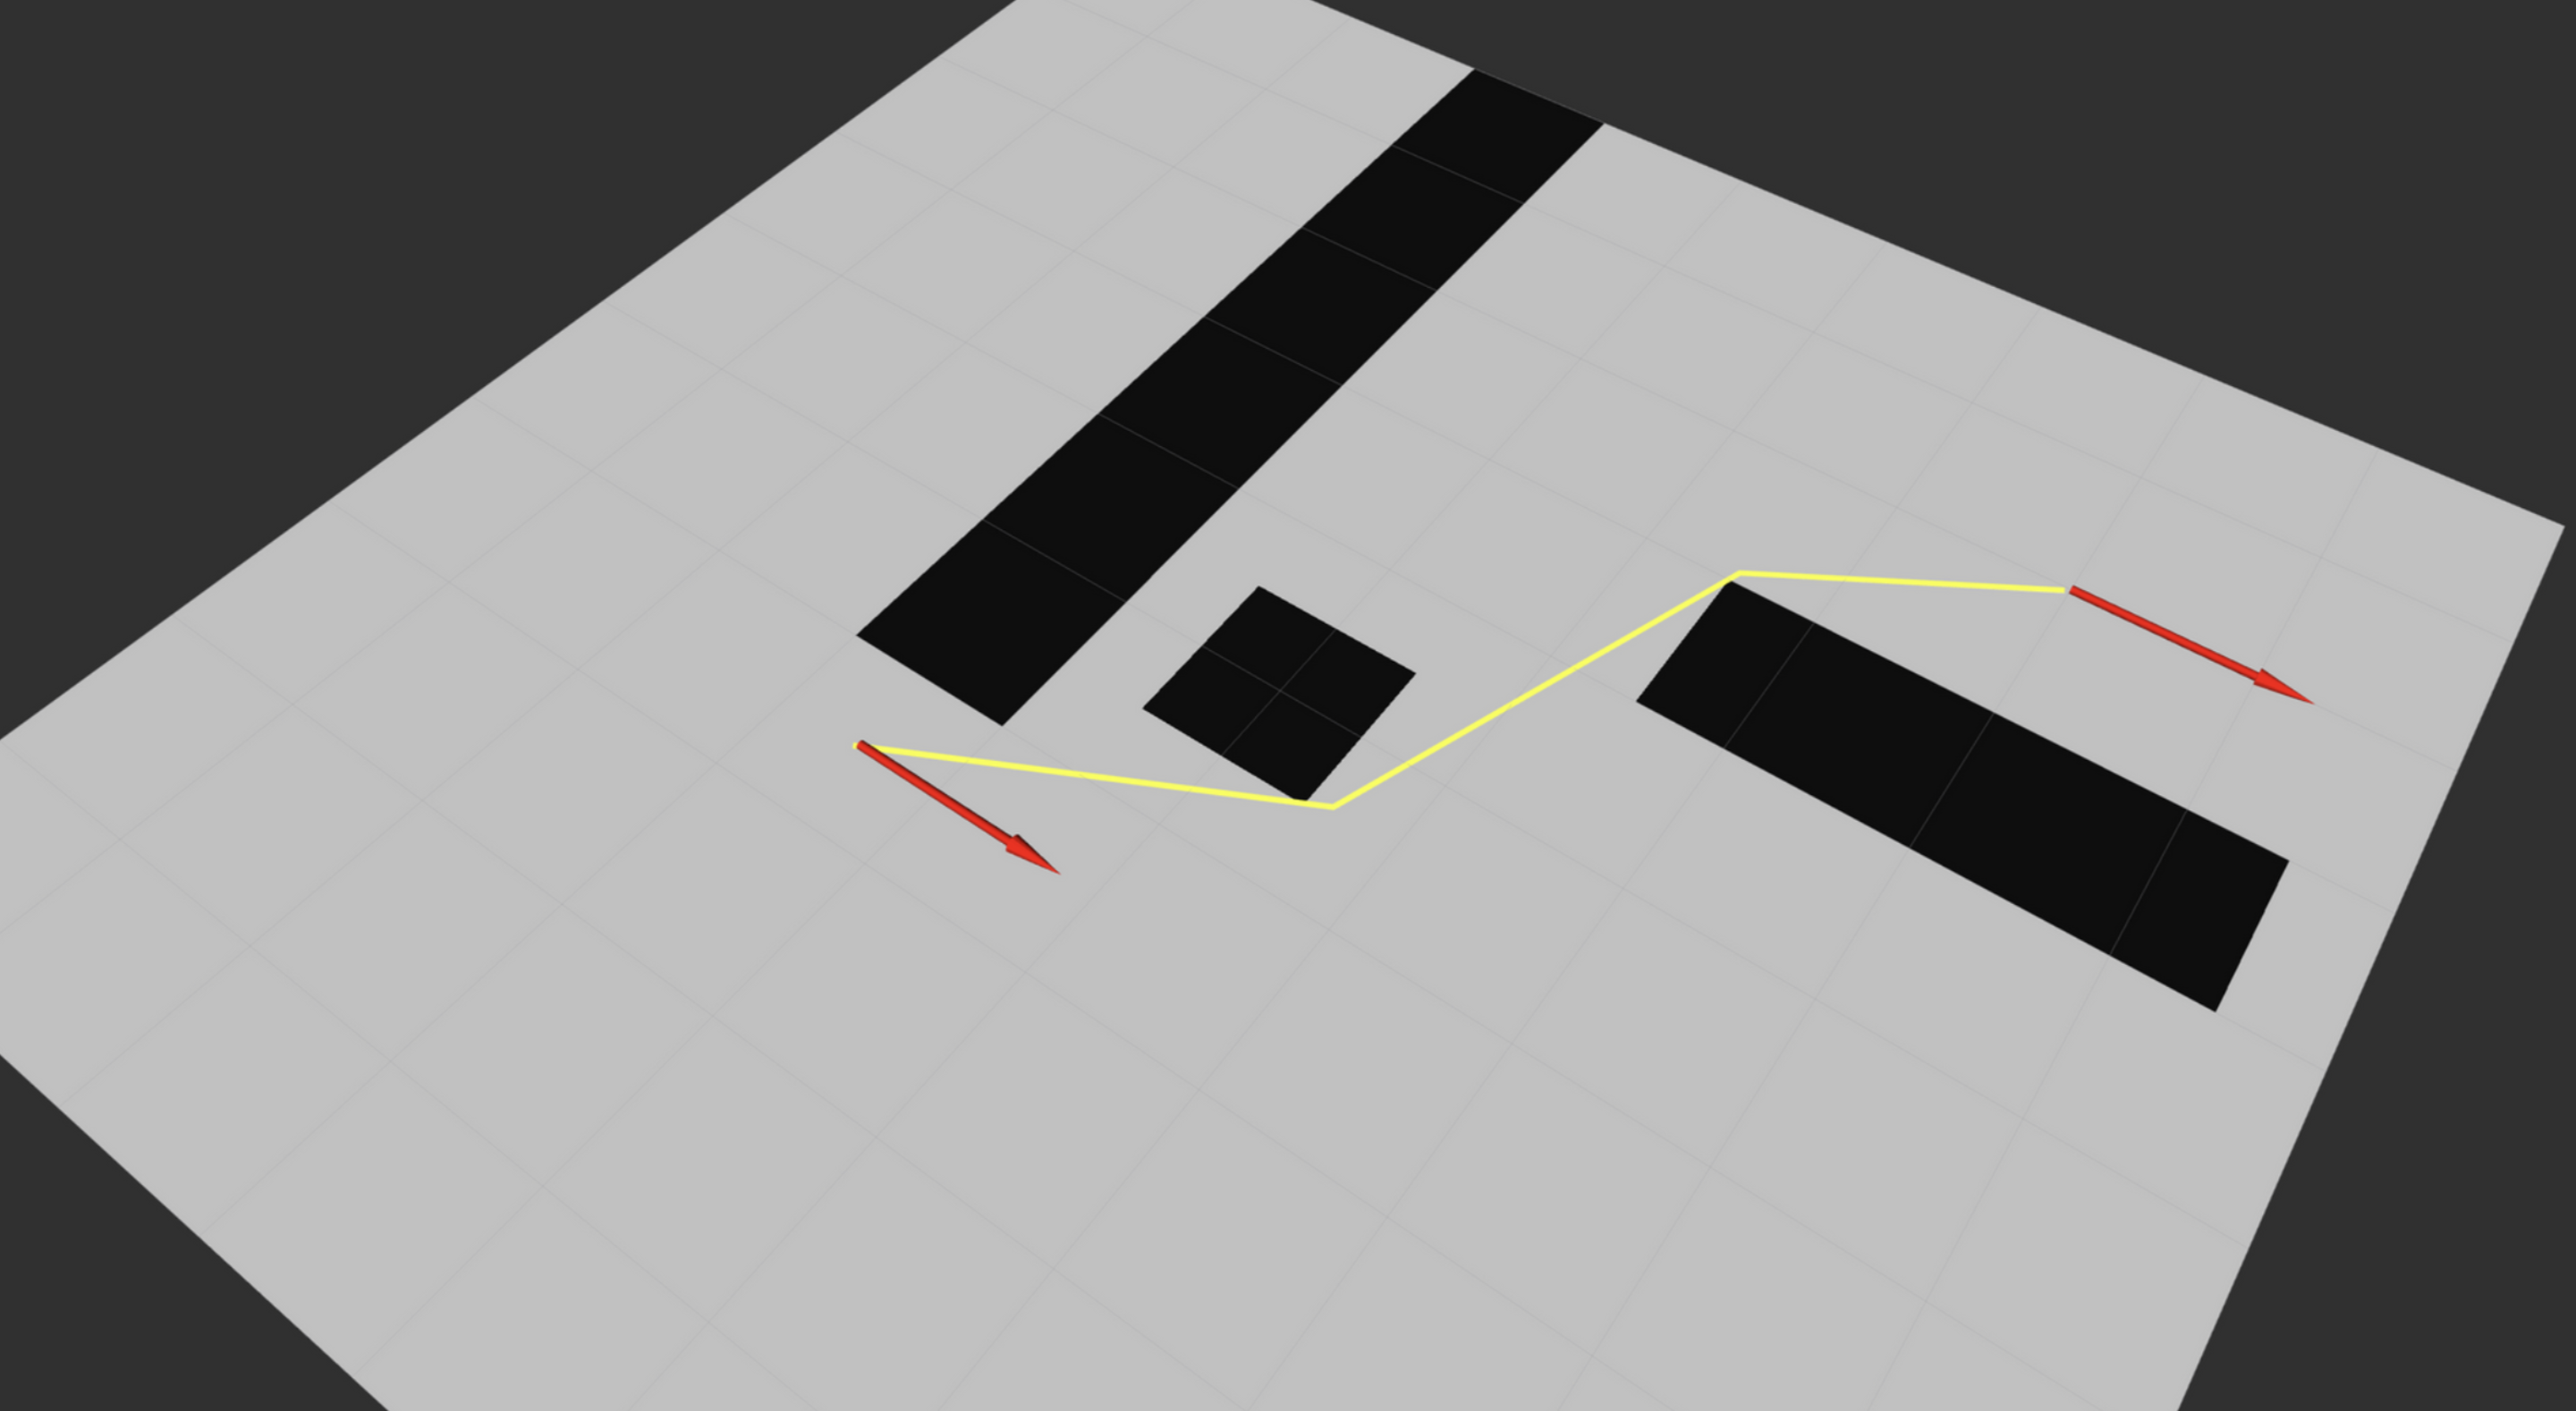
\includegraphics[width=\linewidth]{Images/path2.png}
  \end{minipage}
  \caption{Initial pathfinding: left—raw A* solution; right—after line-of-sight pruning.}
  \label{fig:raw-pruned}
\end{figure}

Subsequently, we introduced obstacle inflation to enforce the robot’s safety margin and avoid corner collisions:

\begin{figure}[ht]
  \centering
  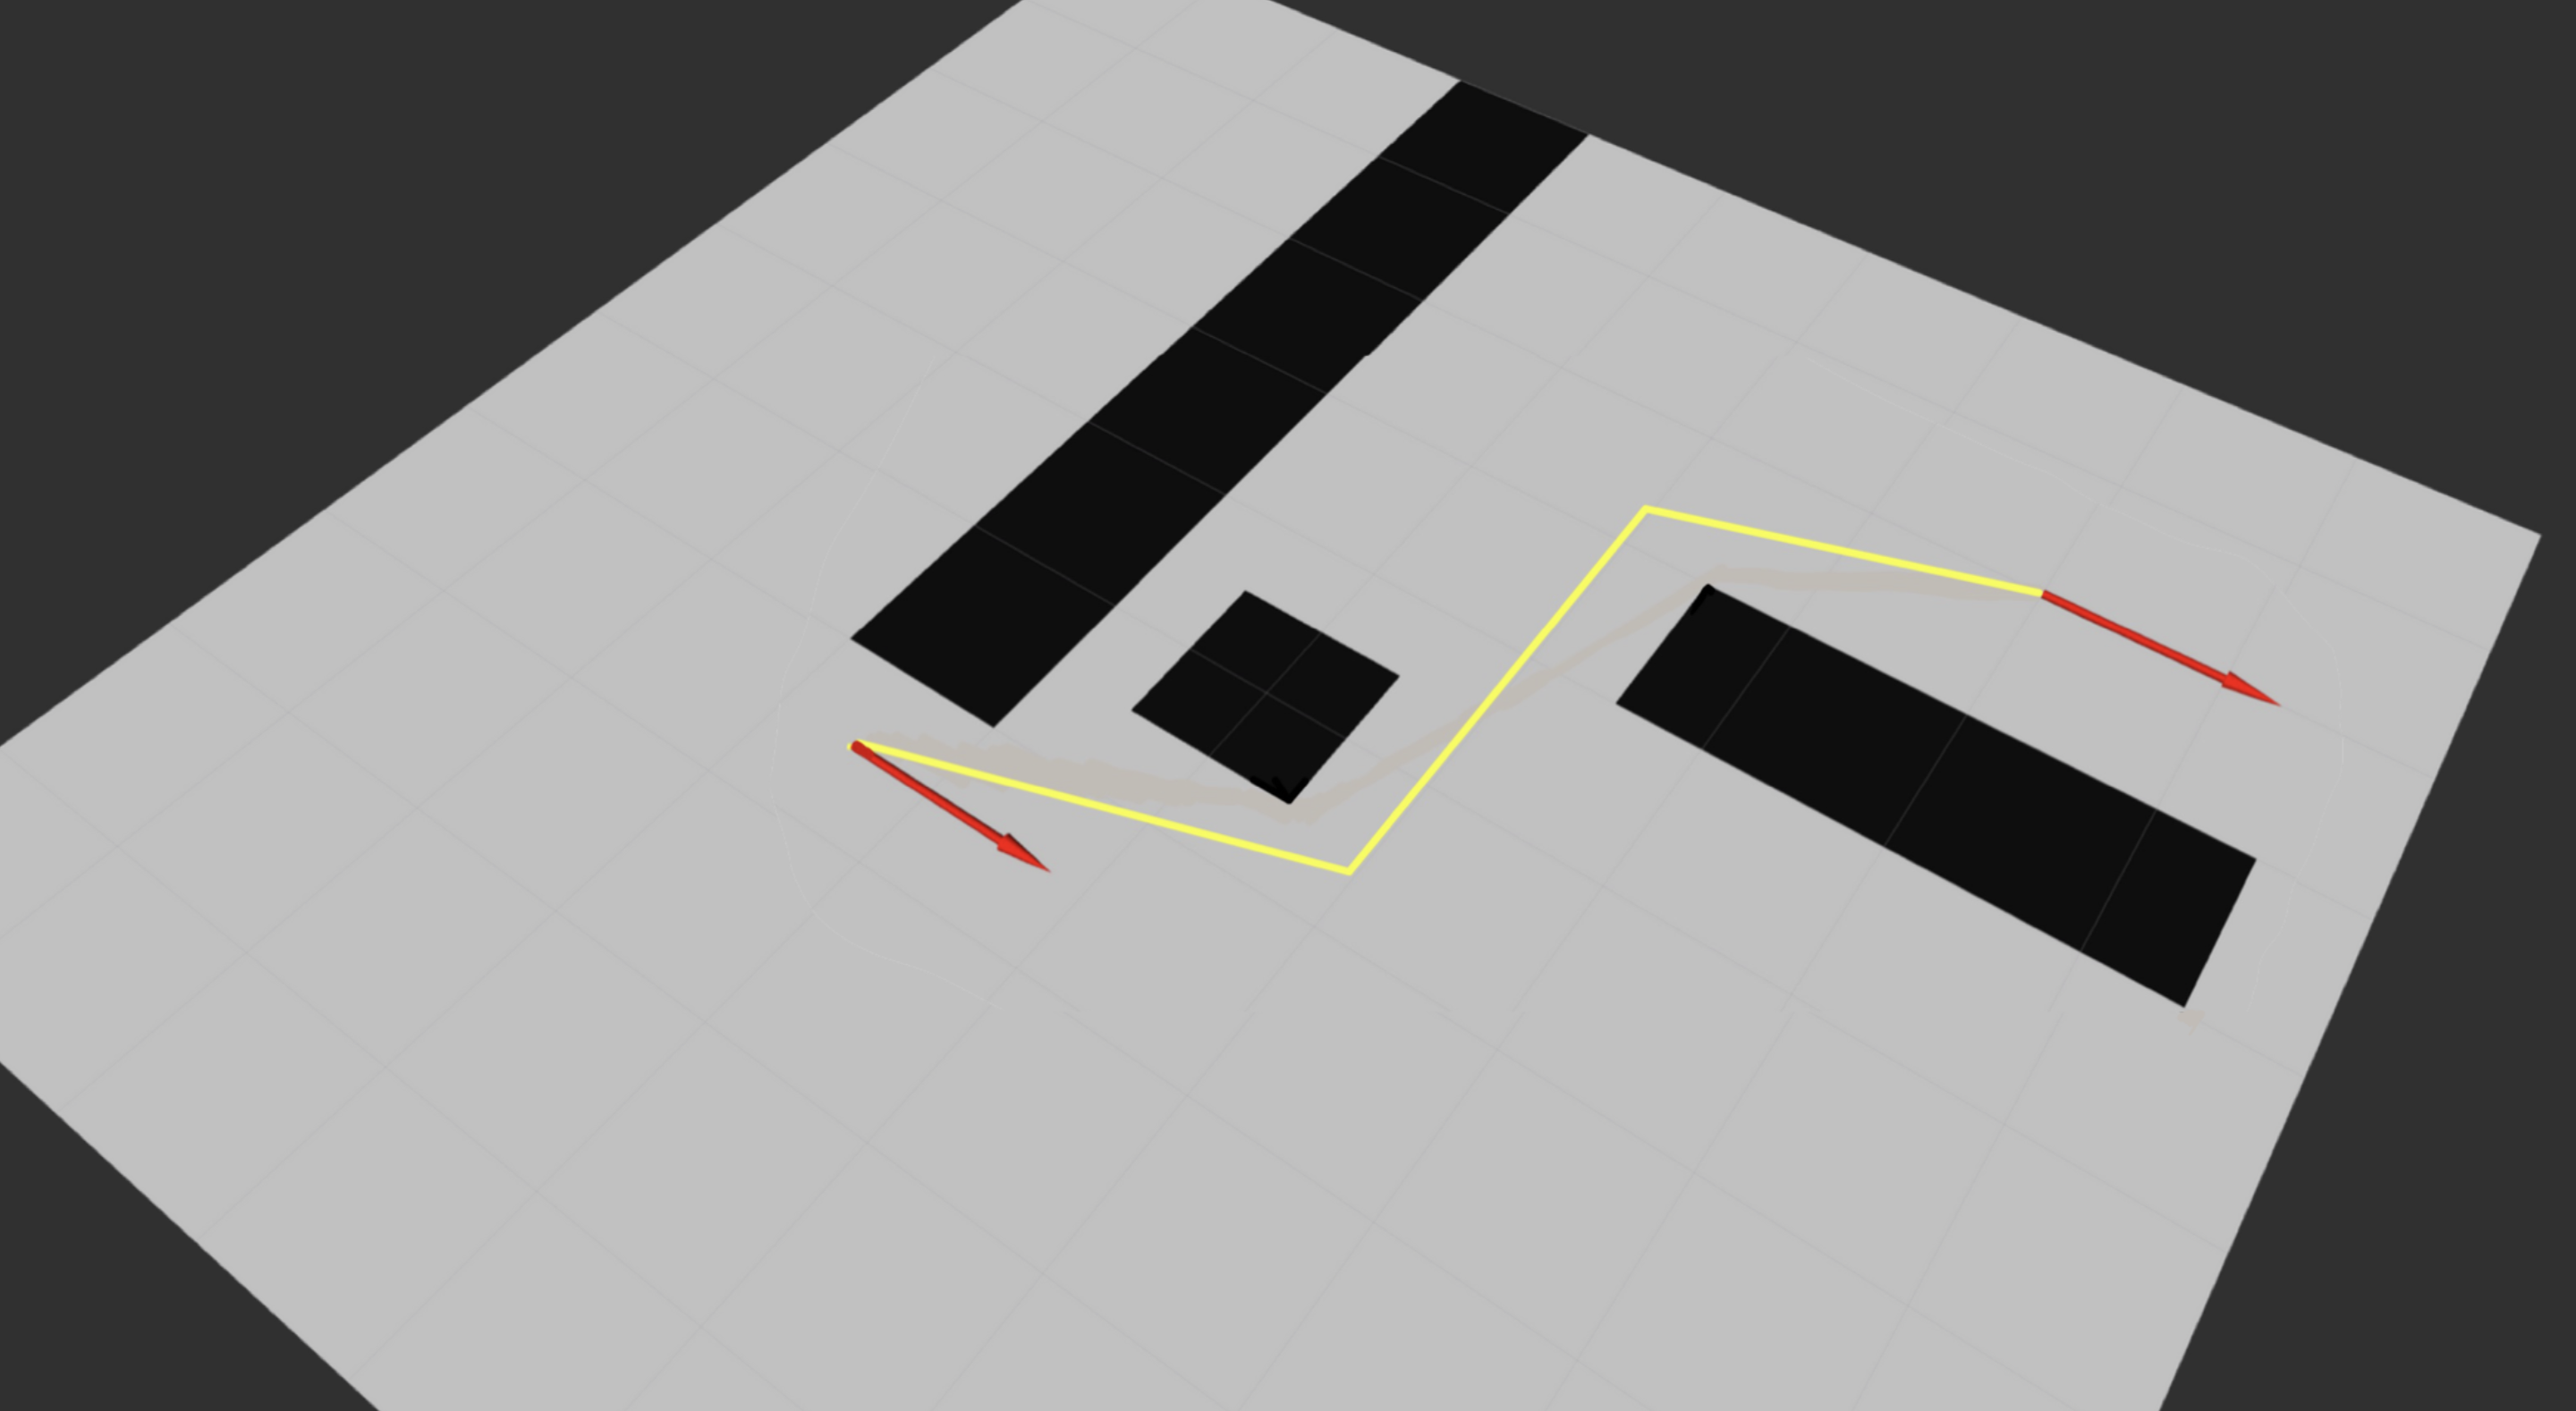
\includegraphics[width=0.4\textwidth]{Images/path3.png}
  \caption{Pathfinding on the inflated map (beige overlay): the planner keeps clear of obstacle edges.}
  \label{fig:inflated}
\end{figure}

\noindent\textbf{Preprocessing steps:}
\begin{itemize}
  \item Reshape \texttt{OccupancyGrid.data} into a 2D array.
  \item Inflate each occupied cell by 
    \texttt{inflate\_radius = int(0.3 / resolution)} 
    to mark neighboring cells as occupied, ensuring collision clearance.
\end{itemize}

\subsubsection{ROS2 Integration}
The planner is implemented as a ROS 2 node with:
\begin{description}
  \item[Subscriptions:] 
    \texttt{/map} (\texttt{OccupancyGrid}), 
    \texttt{/goal\_pose} (\texttt{PoseStamped}), 
    \texttt{/rm0/odom} (\texttt{Odometry}), 
    \texttt{/go\_again}, \texttt{/goal\_reached} (\texttt{Bool}).
  \item[Publishers:] 
    \texttt{/plan} (\texttt{nav\_msgs/Path}), 
    \texttt{/current\_pose} (\texttt{PoseStamped}), 
    \texttt{/rm0/cmd\_vel} (\texttt{Twist}), 
    \texttt{/goal\_reached} (\texttt{Bool}).
  \item[TF Broadcast:] emits an \texttt{odom → base\_link} transform each update, plus a \texttt{static\_transform\_publisher} for \texttt{map → odom} to align frames in RViz.
  \item[Namespace handling:] launch with \texttt{--namespace <robot>} so one codebase runs on multiple robots unchanged.
\end{description}

\subsubsection{Issues Encountered \& Troubleshooting}
\begin{description}
  \item[TF frame misalignment] 
    \textit{Symptom:} paths appeared shifted in RViz.  
    \textit{Diagnosis:} no \texttt{map → odom} static transform in \texttt{/tf}.  
    \textit{Solution:} added a \texttt{static\_transform\_publisher} in the launch file to broadcast an identity \texttt{map → odom}.
  \item[Unknown-cell “blockades”] 
    \textit{Symptom:} planner routed through unexplored (–1) cells on SLAM maps.  
    \textit{Diagnosis:} we treated –1 as free in our occupancy threshold.  
    \textit{Solution:} in \texttt{map\_cb}, mark any \texttt{grid[y][x] < 0} as 100 before inflation, treating unknown as occupied.
  \item[Occupied goal cell handling] 
    \textit{Symptom:} when running the tower-knockdown process, the robot sometimes started inside a region forbidden by the inflated map, causing “no path found.”  
    \textit{Diagnosis:} both start and goal cells were disallowed by inflation.  
    \textit{Solution:} implemented \texttt{\_nearest\_free(goal\_cell)}, which performs an orthogonal BFS to locate the closest free cell; we then replace the goal with that cell and replan automatically.
\end{description}


\subsection{Tower Detection and Interaction System}\label{sec:orbit}
\input{inputs/subinputs/Raffaele.tex}

\subsection{Weak‑Spot Detection \& Shooting}\label{sec:shooter}
\subsubsection*{Tower Alignment and Targeting System}
The system requires alignment algorithm to be used in order to detect the weak side of the tower which, when working with rectangular bases, simply equates to the largest side. The problem could easily be solved by coloring different sides of the tower or by including a special mark on the target side. This solution would harm the implementation on the long run, as we would always be forced to explicitely distinguish sides by altering the visual properties of towers, leading to more constrained and less realistic results.
\subsubsection*{Alignment Detection}
The method we developed to detect the weak side of the tower makes use of the binary mask already in use to assess the position of the tower. In this case we take advantage of the discretization limits of pixels. The easiest, and surprisingly reliable, method to detect whether the robot is looking at a flat face of the tower relies in fact on the distribution of colored pixels in the mask, in particular around the base of the tower. If the number of continuous colored pixels in the first row of the mask containing any non-black pixel (starting from the bottom) is around as high as the highest number of continous pixels in a row of the mask, we can confidently say we are looking at a flat face of the tower. Visually this would mean that in the binary mask we see a sharp edge at the bottom of the tower, instead of a 'pixelated' line.
\subsubsection*{Sensor-Based Geometric Validation}
Once the robot is confident of being parallel to the largest side of the tower we follow an iterative process in order to turn the robot until it looks straight towards its target. The alignment process follows a systematic approach:
\begin{enumerate}
\item \textbf{Initial Rotation}: Controlled rotation at $\omega_{align} = -0.3$ rad/s to scan for geometric variations
\item \textbf{Asymmetry Detection}: Continuous monitoring of range sensor differences to identify tower edges
\item \textbf{Symmetry Convergence}: Fine positioning adjustments to achieve bilateral sensor equality
\item \textbf{Alignment Correction}: Final correction of the alignment following rotation direction
\end{enumerate}
\subsubsection*{Projectile Launch System}
The \textit{shoot\_tower} state executes the engagement sequence through integration with the CoppeliaSim physics engine. The system calculates projectile spawn position using coordinate transformation:
\begin{align} \mathbf{R} &= \begin{bmatrix} \cos(\psi) & -\sin(\psi) & 0 \\ \sin(\psi) & \cos(\psi) & 0 \\ 0 & 0 & 1 \end{bmatrix} \\ \mathbf{p}_{projectile} &= \mathbf{p}_{robot} + \mathbf{R} \cdot \mathbf{t}_{blaster} \end{align}
where $\psi$ represents the robot's roll angle and $\mathbf{t}_{blaster} = [0.2, 0, 0.2]^T$ meters defines the blaster offset from the robot center.
The projectile receives initial velocity $\mathbf{v}_{projectile} = \mathbf{R} \cdot [3.0, 0.0, 3.0]^T$ m/s, providing forward momentum with upward trajectory compensation for ballistic flight. 
% One high‑level figure showing module layout can go here.

% ====================================================================
\section{System Integration}\label{sec:integration}
\subsection{ROS 2 Node Graph \& Communication Channels}
The communication between the three ROS2 nodes in the system — \texttt{MockMapPublisher}, \texttt{PathPlannerNode}, and \texttt{ControllerNode} — is established through various ROS topics. Here's an overview of their coordination logic:\\
At initialization, the \texttt{MockMapPublisher} and \texttt{PathPlannerNode} nodes sets the internal flag \texttt{self.go\_again = True} and the \texttt{ControllerNode} sets \texttt{self.goal\_reached = False}.
These initial states allow both the \texttt{MockMapPublisher} and \texttt{PathPlannerNode} to begin processing immediately, while the \texttt{ControllerNode} waits for confirmation that a goal has been reached.
During operation, once the \texttt{PathPlannerNode} reaches its goal, it publishes a velocity command \texttt{cmd\_vel = (0.0, 0.0)} to bring the robot to a halt. Then publishes the following message to notify other nodes of goal completion:
\[
    \texttt{self.pub\_goal\_reached.publish(Bool(data=True))}
\]
and sets $\texttt{self.go\_again = False}$ to indicate that no further planning is needed until explicitly requested again.
The \texttt{ControllerNode}, which subscribes to the \texttt{/goal\_reached} topic, receives this message and updates its internal flag ($\texttt{self.goal\_reached = True}$). Upon completing its own task (such as analyzing sensor data or interacting with the tower), it publishes:
\[
\texttt{self.turn\_ended.publish(Bool(data=True))}
\]
on the topic \texttt{/go\_again}.
Both the \texttt{MockMapPublisher} and \texttt{PathPlannerNode}, which subscribe to \texttt{/go\_again}, receive this signal and set $\texttt{self.go\_again = True}$.
This loop allows the system to autonomously progress through a series of goals or states in a coordinated manner.
This design ensures that the map publisher and planner are event-driven and coordinated with the controller logic, enabling robust and synchronized robot behavior across discrete tasks.

\subsection{Integration Strategy and Version Control}
% How modules were stitched together (launch files, CI, git workflow).

\subsection{Observed Failure Modes \& Mitigations}
% Latency issues, interface mismatches, etc.

% ====================================================================
\section{Results}\label{sec:results}
A complete execution demo can be found at \href{https://usi365-my.sharepoint.com/:v:/g/personal/costafr_usi_ch/EVE8wwhO59xGo5FCfr8ZFvoBqFdS82ZzTcjgIl_GgPMrJQ?e=QbyhVj}{this link}.

\subsection{Successful outcomes}
The final implementation of the project is able to produce results matching our initial set of requirements in a satisfactory way. The robot in fact capable of, thorugh path planning, reach the position of all towers on the scene. Once the robot is in the vicinity of the tower it then proceeds to orbit around the perimeter of the target in search of the weak-spot (largest flat side). Finally the robot aligns itself to the face of the tower and the action of shooting a projectile towards it is simulated by creating a sphere with adequate mass and velocity.

\begin{figure}[H]
    \centering
    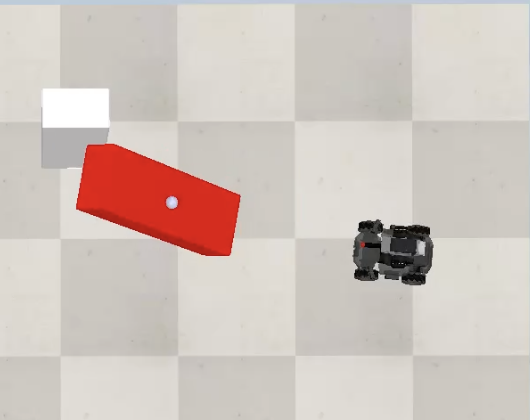
\includegraphics[width=0.3\textwidth]{Images/snapshot_shooting.png}
    \caption{Snapshot of the robot after shooting a projectile.}
    \label{fig:shooting}
\end{figure}

\subsection{Known Issues and Limitations}

While the system fulfils all the baseline requirements, in repeated trials we observed a handful of non‑deterministic failure modes that still require attention:

\begin{itemize}
    \item \textbf{Duplicate \texttt{/goal\_reached} notifications:} Under rare circumstances the topic remains latched and publishes the same message multiple times, leading either to redundant replanning or, conversely, to the node skipping the transition to the next goal.
    \item \textbf{Interleaved sensor callbacks during path execution:} While the robot is orbiting a tower, newly received range data can prompt the planner to generate a fresh trajectory that conflicts with the active controller, producing brief oscillations and jerky motion.
    \item \textbf{Odometry drift after collisions:} Odometry is calculated solely by double‑integrating wheel accelerations; an unexpected collision is therefore interpreted as free motion, causing the estimated pose to diverge from the true pose for the remainder of the run.
    \item \textbf{Weak‑spot detector sensitivity:} Strong glare or partial occlusion can distort the binarisation mask and cause the largest face to be mis‑identified, preventing proper alignment.
\end{itemize}

% ====================================================================
\section{Conclusion \& Future Improvements}\label{sec:conclusion}
\input{inputs/conclusion.tex}


\end{document}